\section{Quellencodierung}
\subsection{Redundanz}
\subsubsection{Codewortlänge $\ell_n$}
\begin{center}
    \begin{tabular}{ c c c }
     Symbol & Code & Codewortlänge \\ 
     $x_0$ & $c_0 = (10)$ & $\ell_0 = 2 Bit$ \\  
     $x_1$ & $c_1 = (110)$ & $\ell_1 = 3 Bit$ \\   
     $x_2$ & $c_2 = (1110)$ & $\ell_2 = 4 Bit$  
    \end{tabular}
\end{center}
\subsubsection{Mittlere Länge der Codierung $L$}
\begin{equation*}
    L = \sum_{n=0}^{N-1} P(x_n) \cdot \ell_n
\end{equation*}
\subsubsection{Redundanz $R$}
In $Bit/Symbol$:
\begin{equation*}
    R = L - H(X)
\end{equation*}
\subsubsection{Theorem zu Quellencodierung}
\begin{itemize}
    \item Falls $R > 0$, dann kann verlustfrei komprimiert werden.
    \item Falls $R \leq 0$, dann kann nur verlustbehaftet komprimiert werden.
\end{itemize}
\subsection{Kompressionsrate}
\begin{align*}
    R = \frac{\text{Grösse Originaldaten}}{\text{Grösse komprimierte Daten}}\\
    \text{Kompressionsrate } R \neq \text{Redundanz } R
\end{align*}
\subsection{Lauflängencodierung}
Lauflängencodierung oder Run-Length Encoding (RLE) ist eine einfache Methode 
zur verlustfreien Datenkompression.
\begin{itemize}
    \item Marker bestimmen, z.B. selten genutzes Zeichen.
    \item Marker und Anzahl der Wiederholungen speichern.
\end{itemize}
\begin{verbatim}
    Hier verwenden wir als Marker z.B. Z:
    Orginal: ASKEEEEEEEEEEFEIIIIIPPPP ...
    Codiert: ASKZ10EZ05IZ04P ...
\end{verbatim}
\subsection{Huffman-Codierung}
Um Huffman-Codierung anzuwenden, muss die Wahrscheinlichkeit $P(x_n)$ der Symbole bekannt sein.
\begin{itemize}
    \item Ordne alle Symbole nach aufsteigenden Auftretenswahrscheinlichkeiten auf einer Zeile. Dies sind die Blätter des Huffman-Baums.
    \item Notiere unter jedes Blatt seine Wahrscheinlichkeit.
    \item Schliesse die beiden Blätter mit der kleinsten Wahrscheinlichkeit an einer gemeinsamen Astgabel an und ordne dem Ast die Summe der Wahrscheinlichkeiten der beiden Blätter zu.
    \item Wiederhole den vorherigen Schritt mit Blättern und Ästen so lange, bis nur noch der Stamm des Baums übrig bleibt.
    \item Nun wird bei jeder Astgabel dem einen Zweig eine 0 und dem anderen eine 1 zugeordnet. (Die Zuordnung ist frei wählbar, muss aber über den ganzen Baum einheitlich sein).
    \item Nun werden auf dem Pfad vom Stamm zu jedem Blatt die Nullen und Einsen ausgelesen und von links nach rechts nebeneinander geschrieben. Dies sind die Huffman-Codeworte.
\end{itemize}
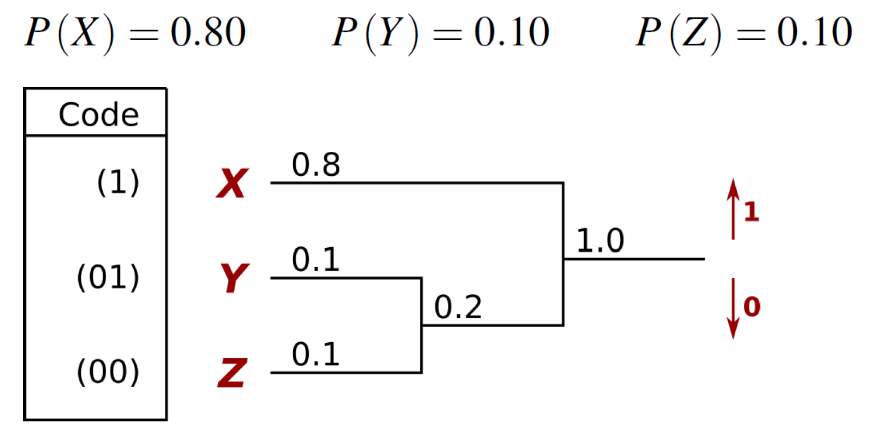
\includegraphics[scale= 0.4]{huffman}
\subsection{LZ77}
Für LZ77 ein Suchbuffer $n_{s}$ und Vorschaubuffer $n_{v}$ definiert.
Der Token hat das Format (Offset, Länge, Zeichen).
\begin{center}
    \begin{tabular}{ c c c c }
        Suchbuffer ($n_{s}$) & Vorschaubuffer ($n_{v}$) & Restdaten & Token \\ 
        ... & ... & ... & ... \\  
        ... & ... & ... & ... \\  
        ... & ... & ... & ... \\  
        ... & ... & ... & ... \\  
        ... & ... & ... & ... \\  
    \end{tabular}
\end{center}
\subsection{LZW}

